% CS765 Aspects of System Administration
% Author: Jan Schaumann <jschauma@netmeister.org>
% $Id: slides.tex,v 1.7 2004/07/06 20:05:22 jschauma Exp $
\special{! TeXDict begin /landplus90{true}store end }

\documentclass[xga]{xdvislides}
\usepackage[landscape]{geometry}
\usepackage{graphics}
\usepackage{graphicx}
\usepackage{colordvi}

\begin{document}
\setfontphv

%%% Headers and footers
\lhead{\slidetitle}                               % default:\lhead{\slidetitle}
\chead{CS765 - Aspects of System Administration}% default:\chead{\relax}
\rhead{Slide \thepage}                       % default:\rhead{\sectiontitle}
\lfoot{\Gray{System Security}}% default:\lfoot{\slideauthor}
\cfoot{\relax}                               % default:\cfoot{\relax}
\rfoot{\Gray{\today}}
\vspace*{\fill}
\begin{center}
	\Hugesize
		CS615 - Aspects of System Administration\\ [1em]
		System Security\\ [1em]
	\hspace*{5mm}\blueline\\ [1em]
	\Normalsize
		Department of Computer Science\\
		Stevens Institute of Technology\\
		Jan Schaumann\\
		\verb+jschauma@stevens.edu+ \\
		\verb+http://www.cs.stevens.edu/~jschauma/615/+
\end{center}
\vspace*{\fill}

\subsection{Where/how does 'security' come into play?}

\subsection{Where/how does 'security' come into play?}
Lecture 02 (Filesystems, Disks, Storage)
\begin{itemize}
	\item storage model (DAS, NAS, SAN, Cloud)
	\item partitions / mount options
	\item filesystem features (permissions, access control lists)
\end{itemize}
\vspace{.5in}
Lecture 03 (Software Installation Concepts)
\begin{itemize}
	\item boot sequence, firmware
	\item OEM added software (Superfish)
	\item software package management and updates
	\item patch management
\end{itemize}

\subsection{Where/how does 'security' come into play?}
Lecture 04 (Packaging, Multiuser Fundamentals, Ethics)
\begin{itemize}
	\item Xen vulnerabilities
	\item vulnerability tracking
	\item privileges and trust models
	\item privacy, obligation to protect users, social responsibility
\end{itemize}
\vspace{.5in}
Lecture 05 (Automation)
\begin{itemize}
	\item FREAK attack (CVE-2015-0204)
	\item using the wrong tool for the job => writing insecure code
	\item understanding language / framework pitfalls
\end{itemize}

\subsection{Where/how does 'security' come into play?}
Lecture 06 (Networking)
\begin{itemize}
	\item network censorship
	\item protocols and visibility of data on different layers
	\item tcpdump can read all packets
	\item location of attacker on network implies capabilities
\end{itemize}
\vspace{.5in}
Lecture 07 (Backup and Disaster Recovery)
\begin{itemize}
	\item DDoS attack on GitHub / GreatFire.org
	\item disasters include security breaches
	\item safety of backups (encrypted backups?)
\end{itemize}

\subsection{Where/how does 'security' come into play?}
Lecture 08 (DNS)
\begin{itemize}
	\item traffic censorship
	\item DNS registrars as attack points
	\item use of DNS as another channel for host verification (SSHFP records)
	\item trustworthiness of DNS (DNSSEC)
\end{itemize}
\vspace{.5in}
Lecture 09 (SMTP, HTTP)
\begin{itemize}
	\item email as attack methods (spam, phishing)
	\item email privacy implications
	\item email relaying
	\item HTTP as universal network entry point
	\item HTTP fronting applications and handling data
\end{itemize}

\subsection{Where/how does 'security' come into play?}
Lecture 10 (SSH)
\begin{itemize}
	\item Confidentiality, Integrity, Authenticity
	\item threat modeling
	\item asymmetric encryption
\end{itemize}
\vspace{.5in}
Lecture 11 (Monitoring, SNMP)
\begin{itemize}
	\item availability of logs to establish context
	\item sensitive data in logs
	\item outsourcing monitoring services
\end{itemize}

\subsection{How do we secure a system?}

\subsection{How do we secure a system?}
\Huge
\vspace*{\fill}
\begin{center}
	It depends. \\
\vspace{.5in}
\Normalsize
	(Context required.)
\end{center}
\vspace*{\fill}

\subsection{What is security?}
\Huge
\begin{verbatim}
security

 NOUN:

   Freedom from risk or danger; safety.
\end{verbatim}
\Normalsize

\subsection{What is risk?}
\Huge
\begin{verbatim}
risk

 NOUN:

  The possibility of suffering harm or loss; danger.
\end{verbatim}
\Normalsize

\subsection{Suffering harm or loss of {\em what}?}

\begin{itemize}
	\item access to data
\end{itemize}

\subsection{Suffering harm or loss of {\em what}?}

\begin{itemize}
	\item access to data
	\item integrity of data
\end{itemize}

\subsection{Suffering harm or loss of {\em what}?}

\begin{itemize}
	\item access to data
	\item integrity of data
	\item availability of services
\end{itemize}

\subsection{Suffering harm or loss of {\em what}?}

\begin{itemize}
	\item access to data
	\item integrity of data
	\item availability of services
	\item reputation
\end{itemize}

\subsection{Suffering harm or loss of {\em what}?}

\begin{itemize}
	\item access to data
	\item integrity of data
	\item availability of services
	\item reputation
	\item monetary loss due to any of the above
\end{itemize}

\subsection{Suffering harm or loss of {\em what}?}

\begin{itemize}
	\item access to data
	\item integrity of data
	\item availability of services
	\item reputation
	\item monetary loss due to any of the above
	\item monetary loss due to physical items of actual value
\end{itemize}

\subsection{Suffering harm or loss of {\em what}?}

\begin{itemize}
	\item access to data
	\item integrity of data
	\item availability of services
	\item reputation
	\item monetary loss due to any of the above
	\item monetary loss due to physical items of actual value
	\item ...
\end{itemize}


\subsection{How to determine {\em risk}}
``Risk Assessment''
\begin{itemize}
	\item identify {\em assets}
\end{itemize}

\subsection{How to determine {\em risk}}
``Risk Assessment''
\begin{itemize}
	\item identify {\em assets}
	\item identify {\em threats}
\end{itemize}


\subsection{How to determine {\em risk}}
``Risk Assessment''
\begin{itemize}
	\item identify {\em assets}
	\item identify {\em threats}
	\item identify {\em vulnerabilities}
\end{itemize}

\subsection{How to determine {\em risk}}
``Risk Assessment''
\begin{itemize}
	\item identify {\em assets}
	\item identify {\em threats}
	\item identify {\em vulnerabilities}
	\item determine {\em likelihood of damage}
\end{itemize}

\subsection{How to determine {\em risk}}
``Risk Assessment''
\begin{itemize}
	\item identify {\em assets}
	\item identify {\em threats}
	\item identify {\em vulnerabilities}
	\item determine {\em likelihood of damage}
	\item estimate {\em cost of recovery}
\end{itemize}

\subsection{How to determine {\em risk}}
``Risk Assessment''
\begin{itemize}
	\item identify {\em assets}
	\item identify {\em threats}
	\item identify {\em vulnerabilities}
	\item determine {\em likelihood of damage}
	\item estimate {\em cost of recovery}
	\item estimate {\em cost of defense}
\end{itemize}

\subsection{How to determine {\em risk}}
``Risk Assessment''
\begin{itemize}
	\item identify {\em assets}
	\item identify {\em threats}
	\item identify {\em vulnerabilities}
	\item determine {\em likelihood of damage}
	\item estimate {\em cost of recovery}
	\item estimate {\em cost of defense}
\end{itemize}
\vspace{.5in}

A {\em risk} is the {\em likelihood} of a {\em threat} successfully exploiting
a {\em vulnerability} and the {\em estimated cost} (or potential damage) both
in the short and long term you may incur as a result.

\subsection{Threat Model}
For each system/component/product/service/...

\begin{itemize}
	\item identify {\em what} you're protecting
	\item identify {\em whom} you're protecting it {\em from}
		\begin{itemize}
			\item identify {\em goals} of the attacker
			\item identify {\em motivation} of the attacker
			\item identify {\em capabilities} of the attacker
		\end{itemize}
	\item identify threats you cannot defend against (within this
		system or in general)
\end{itemize}

\subsection{Defense in Depth}
\vspace*{\fill}
\Huge
\begin{center}
	Security is like an onion: \\
	the more layers you peel away, the more it stinks.
\end{center}
\Normalsize
\vspace*{\fill}

\subsection{The biggest threat comes from the inside}
\vspace*{\fill}
\begin{center}
	
\includegraphics[scale=1.0]{pics/kane.eps}
\end{center}
\vspace*{\fill}

\subsection{The biggest threat comes from the inside}
\vspace*{\fill}
\begin{center}
	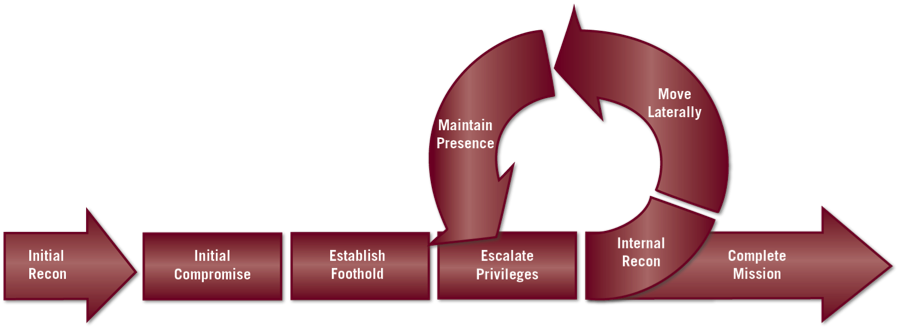
\includegraphics[scale=1.0]{pics/Killchain.eps} \\
	\verb+http://is.gd/6sREQh+
\end{center}
\vspace*{\fill}

\subsection{Cryptography}
\Normalsize
{\em Cryptography} can help mitigate {\em some} of the risks {\em sometimes}.

\subsection{Cryptography}
{\em Cryptography} can help mitigate {\em some} of the risks {\em sometimes}.
\\

It may provide security in the areas of:
\begin{itemize}
	\item Secrecy or Confidentiality
		\begin{itemize}
			\item {\em Did/could anybody else see (parts of) the message?}
		\end{itemize}
\end{itemize}

\subsection{Cryptography}
{\em Cryptography} can help mitigate {\em some} of the risks {\em sometimes}.
\\

It may provide security in the areas of:
\begin{itemize}
	\item Secrecy or Confidentiality
		\begin{itemize}
			\item {\em Did/could anybody else see (parts of) the message?}
		\end{itemize}
	\item Accuracy or Integrity
		\begin{itemize}
			\item {\em Was the message (could it have been) modified before I received it?}
		\end{itemize}
\end{itemize}

\subsection{Cryptography}
{\em Cryptography} can help mitigate {\em some} of the risks {\em sometimes}.
\\

It may provide security in the areas of:
\begin{itemize}
	\item Secrecy or Confidentiality
		\begin{itemize}
			\item {\em Did/could anybody else see (parts of) the message?}
		\end{itemize}
	\item Accuracy or Integrity
		\begin{itemize}
			\item {\em Was the message (could it have been) modified before I received it?}
		\end{itemize}
	\item Authenticity
		\begin{itemize}
			\item {\em Is the party I'm talking to actually
who I think it is / they claim they are?}
		\end{itemize}
\end{itemize}

\subsection{Cryptography}
Note:
\begin{itemize}
	\item {\em Authentication} \verb+!=+ {\em Authorization}
	\item cryptography does not handle authorization
	\item you generally need all three: confidentiality, integrity, authenticity
	\item cryptography cannot prevent against incorrect use \\
		(usability is hard, let's go shopping)
\end{itemize}
\addvspace{.5in}
Know your threat model!

\subsection{Basic Security Concepts: Confidentiality}
\begin{itemize}
	\item Alice and Bob agree on a way to transform plain text into ciphertext
	\item transformed data is sent over insecure channel
	\item Alice and Bob are able to reverse transformation
\end{itemize}

\subsection{Basic Security Concepts: Confidentiality}
\begin{itemize}
	\item Alice and Bob agree on a way to transform plain text into ciphertext
	\item transformed data is sent over insecure channel
	\item Alice and Bob are able to reverse transformation
\end{itemize}
\addvspace{.5in}
Different approaches:
\begin{itemize}
	\item secret key cryptography (example: {\em DES})
		\begin{itemize}
			\item Alice and Bob share a secret key
		\end{itemize}
\end{itemize}
\addvspace{.25in}
\begin{itemize}
	\item public key cryptography (example: {\em RSA})
		\begin{itemize}
			\item Alice has a private and a public key
			\item data encrypted with her private key can only be decrypted by
				her public key and vice versa
			\item public key can be shared with anybody (via insecure means)
		\end{itemize}
\end{itemize}

\subsection{Threats to Confidentiality}
\begin{itemize}
	\item lack of {\em authenticity}
	\item key exchange
	\item key disclosure
\end{itemize}

\subsection{Basic Security Concepts: Integrity}
In order to protect against forgery or data manipulation, provide some sort of
digest or checksum (often a one-way hash).  Popular choices:

\begin{itemize}
	\item {\tt 5f4dcc3b5aa765d61d8327deb882cf99}
	\item {\tt 5baa61e4c9b93f3f0682250b6cf8331b7ee68fd8}
	\item {\tt 5e884898da28047151d0e56f8dc6292773603d0d6aabbdd62 \
                   a11ef721d1542d8}
	\item {\tt b109f3bbbc244eb82441917ed06d618b9008dd09b3befd1b5 \
                   e07394c706a8bb980b1d7785e5976ec049b46df5f1326af5a \
                   2ea6d103fd07c95385ffab0cacbc86}
\end{itemize}

\subsection{Basic Security Concepts: Integrity}
In order to protect against forgery or data manipulation, provide some sort of
digest or checksum (often a one-way hash).  Popular choices:

\begin{itemize}
	\item {\tt 5f4dcc3b5aa765d61d8327deb882cf99} (MD5)
	\item {\tt 5baa61e4c9b93f3f0682250b6cf8331b7ee68fd8} (SHA-1)
	\item {\tt 5e884898da28047151d0e56f8dc6292773603d0d6aabbdd62 \
                   a11ef721d1542d8} (SHA256)
	\item {\tt b109f3bbbc244eb82441917ed06d618b9008dd09b3befd1b5 \
                   e07394c706a8bb980b1d7785e5976ec049b46df5f1326af5a \
                   2ea6d103fd07c95385ffab0cacbc86} (SHA512)
\end{itemize}

\subsection{Basic Security Concepts: Integrity}
Examples: host based IDS, package manager signatures

\vspace{.5in}
Some possible threats:
\begin{itemize}
	\item collisions in algorithm
	\item lack of {\em authenticity} (Where did I get the checksum?)
	\item lack of {\em integrity} (Was the checksum tampered to match the (tampered) data?)
	\item ``verification'' with compromised tools
	\item ``rainbow tables'' / internet search engines allow for easy reverse
		lookup of un-salted hashes.
\end{itemize}

\subsection{Basic Security Concepts: Authenticity}
Three general ways of proving that you are who you say you are:
\begin{itemize}
	\item something you know
	\item something you have
	\item something you are
\end{itemize}

\subsection{Basic Security Concepts: Authenticity}
Three general ways of proving that you are who you say you are:
\begin{itemize}
	\item something you know
		\begin{itemize}
			\item secret handshake, password
			\item can (easily) be given to and used by somebody else
		\end{itemize}
	\item something you have
	\item something you are
\end{itemize}

\subsection{Basic Security Concepts: Authenticity}
Three general ways of proving that you are who you say you are:
\begin{itemize}
	\item something you know
		\begin{itemize}
			\item secret handshake, password
			\item can (easily) be given to and used by somebody else
		\end{itemize}
	\item something you have
		\begin{itemize}
			\item physical items: smart card, RSA token, ...
			\item private keys
			\item can (easily) be given to and used by somebody else
		\end{itemize}
	\item something you are
\end{itemize}

\subsection{Basic Security Concepts: Authenticity}
Three general ways of proving that you are who you say you are:
\begin{itemize}
	\item something you know
		\begin{itemize}
			\item secret handshake, password
			\item can (easily) be given to and used by somebody else
		\end{itemize}
	\item something you have
		\begin{itemize}
			\item physical items: smart card, RSA token, ...
			\item private keys
			\item can (easily) be given to and used by somebody else
		\end{itemize}
	\item something you are
		\begin{itemize}
			\item physical, physiological or behavioral traits
			\item can not (easily or at all) be given to or
				used by somebody else
		\end{itemize}
\end{itemize}

\subsection{Basic Security Concepts: Authenticity}
Some possible threats:
\begin{itemize}
	\item lack of {\em confidentiality}
	\item lack of {\em integrity}
	\item reliance on fragile infrastructure
	\item usability
	\item conflation with {\em authorization}
\end{itemize}

\subsection{Principle of Least Privilege}
\vspace*{\fill}
\begin{center}
	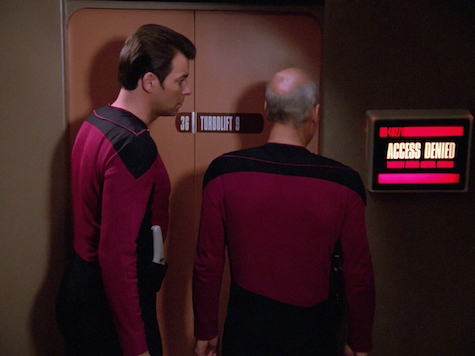
\includegraphics[scale=0.9]{pics/turbolift_access_denied.eps}
\end{center}
\vspace*{\fill}

\subsection{It's not just 1s and 0s}
\vspace{.5in}
\Huge
\begin{center}
System security is not restricted to {\em software} security.
\end{center}
\Normalsize

\subsection{It's not just 1s and 0s}
\vspace{.5in}
\Huge
\begin{center}
The thing that makes security difficult is not the software or hardware
components.  It's the human component.
\end{center}
\Normalsize

\subsection{It's not just 1s and 0s}
\vspace*{\fill}
\begin{center}
	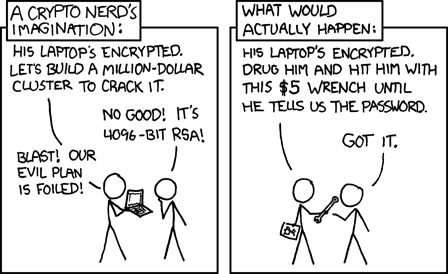
\includegraphics[scale=1.3]{pics/security.eps}
\end{center}
\vspace*{\fill}



\subsection{Secure by default}
\vspace{.5in}
\Huge
\begin{center}
Users care about usability, not about security.
\end{center}
\Normalsize

\subsection{Secure by default}
\vspace{.5in}
\Huge
\begin{center}
Users will not change their default settings.
\end{center}
\Normalsize

\subsection{Secure by default}
\vspace{.5in}
\Huge
\begin{center}
Users will not change their default settings. \\
\Normalsize
(Unless a less secure option is available.)
\end{center}

\newpage
\vspace*{\fill}
\begin{center}
    \Hugesize
        Hooray! \\ [1em]
    \hspace*{5mm}
    \blueline\\
    \hspace*{5mm}\\
        5 Minute Break
\end{center}
\vspace*{\fill}

\subsection{Security Fallacies and Pitfalls}
\vspace*{\fill}
\begin{center}
    \Hugesize
        Proving a Negative \\
	\vspace{.25in}
	\Normalsize
	(Evidence of Absences vs. Absence of Evidence)
\end{center}
\vspace*{\fill}


\subsection{Security Fallacies and Pitfalls}
\vspace*{\fill}
\begin{center}
    \Hugesize
        Security by Obscurity
\end{center}
\vspace*{\fill}

\subsection{Security Fallacies and Pitfalls}
\vspace*{\fill}
\begin{center}
    \Hugesize
        Perfect is the Enemy of the Good \\
	\vspace{.25in}
	\Normalsize
	(Differentiate between futile efforts and raising the bar.)
\end{center}
\vspace*{\fill}

\subsection{Security Fallacies and Pitfalls}
\vspace*{\fill}
\begin{center}
    \Hugesize
        One in a million is next Tuesday. \\
	\vspace{.25in}
	\Normalsize
	\verb+http://is.gd/Isb20K+
\end{center}
\vspace*{\fill}

\subsection{Security Fallacies and Pitfalls}
\vspace*{\fill}
\begin{center}
    \Hugesize
        ``Any person can invent a security system so clever that she or he
can't think of how to break it.'' \\
	\vspace{.25in}
	\Normalsize
	Schneier's Law \verb+http://is.gd/hW82dt+
\end{center}
\vspace*{\fill}

\subsection{Security Fallacies and Pitfalls}
\vspace*{\fill}
\begin{center}
    \Hugesize
        Don't invent your own crypto. \\
	\vspace{.25in}
	\Normalsize
	(Seriously, don't.)
\end{center}
\vspace*{\fill}

\subsection{Security Fallacies and Pitfalls}
\vspace*{\fill}
\begin{center}
    \Hugesize
	Complexity is the worst enemy of security. \\
	\vspace{.25in}
	\Normalsize
	(The more secure you make something, the less secure it becomes.)
\end{center}
\vspace*{\fill}

\subsection{Whom do you trust?}
\vspace*{\fill}
\begin{center}
	\verb+http://cm.bell-labs.com/who/ken/trust.html+
\end{center}
\vspace*{\fill}
\Normalsize

\subsection{Outsourcing Services}
\begin{itemize}
	\item you trust the provider/vendor to honor the agreement
	\item you ``hope'' they won't change their agreement (once
		invested, changing back is hard)
	\item you trust the provider/vendor to keep their infrastructure
		safe
	\item you trust the provider/vendor's employees
	\item you are ok with the traffic going across the public internet
\end{itemize}

\subsection{Toning down the Paranoia}
\vspace*{\fill}
\Huge
\begin{center}
Never attribute to malice that which can be adequately explained by stupidity. \\
\vspace{.25in}
\Normalsize
Hanlon's Razor
\end{center}
\Normalsize
\vspace*{\fill}

\subsection{Sysadmin $\cap$ Infosec}
\vspace*{\fill}
\begin{center}
	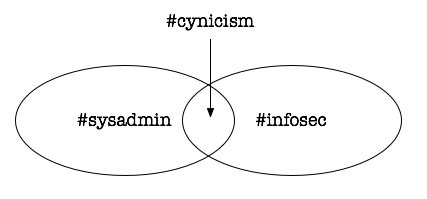
\includegraphics[scale=1.0]{pics/sysadmin_infosec.eps} \\
	\verb+https://www.netmeister.org/blog/infosec-basics.html+
\end{center}
\vspace*{\fill}

\subsection{Sysadmin $\cap$ Infosec}
\vspace*{\fill}
\Huge
\begin{center}
	Nothing is always absolutely so.
\end{center}
\Normalsize
\vspace*{\fill}

\subsection{Two Questions}
\vspace*{\fill}
\begin{center}
	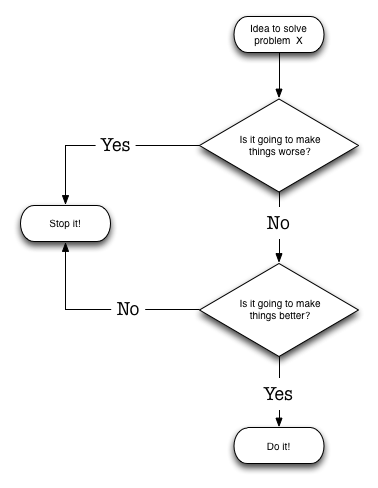
\includegraphics[scale=0.67]{pics/two-questions.eps} \\
\small
	\verb+https://www.netmeister.org/blog/two-questions.html+
\end{center}
\Normalsize
\vspace*{\fill}

\subsection{HW6}
\vspace*{\fill}
\begin{center}
	\verb+https://www.cs.stevens.edu/~jschauma/615/s15-ctf.html+
\end{center}
\Normalsize
\vspace*{\fill}

\end{document}
